\begin{center}
    \begin{tikzpicture}[] 
        \node[] at (-4, 0) (cam) {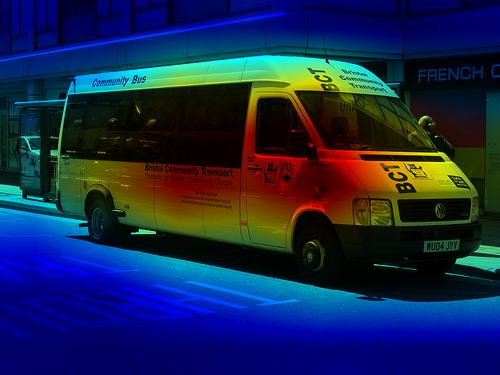
\includegraphics[width=.33\textwidth]{fig/castream/img/Comparable/figure1/gradcam/27079}};
        \node[] at (-4, 1.5) (camtxt) {\scriptsize Saliency Maps};
        \pause
        \node[] at (0, 0) (grad) {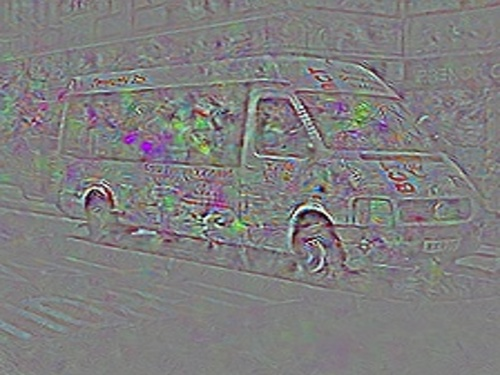
\includegraphics[width=.33\textwidth]{fig/intro/comp_cv_ai/img/gb_van}};
        \node[] at (0, 1.5) (gradtxt) {\scriptsize Gradients};
        \pause
        \node[] at (3.5, .5) (wshld) {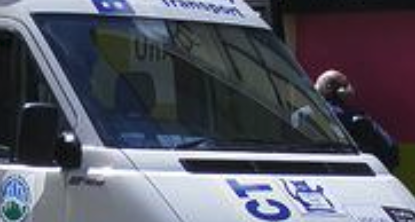
\includegraphics[scale=.125]{fig/intro/comp_cv_ai/img/parts_van/wshld.png}};
        \node[] at (4, 1.5) (other) {\scriptsize Other Representations};
        \node[] at (wshld.south east) (lights) {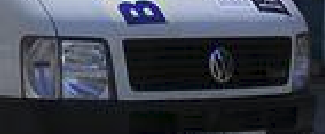
\includegraphics[scale=.125]{fig/intro/comp_cv_ai/img/parts_van/lights.png}};
        \node[] at (lights.south west) (front) {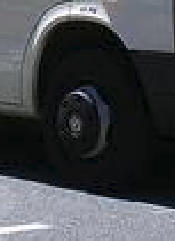
\includegraphics[scale=.125]{fig/intro/comp_cv_ai/img/parts_van/front.png}};
        \node[] at (front.west) {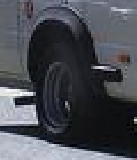
\includegraphics[scale=.125]{fig/intro/comp_cv_ai/img/parts_van/rear.png}};
        \pause
        \node[rectangle, opacity=1, draw=red, minimum width=8cm, minimum height=2.75cm, very thick] at (-2, 0) (rect_chosen) {};
        \node at (-1.5, -1.75) {\scriptsize We demonstrate improvements in these approaches};
    \end{tikzpicture}    
\end{center}
